%----------------------------------------------------------------------------------------
%	SPACEWEATHER EVENT.
%----------------------------------------------------------------------------------------
\section{Space weather event}
\begin{wrapfigure}[18]{r}{6cm}
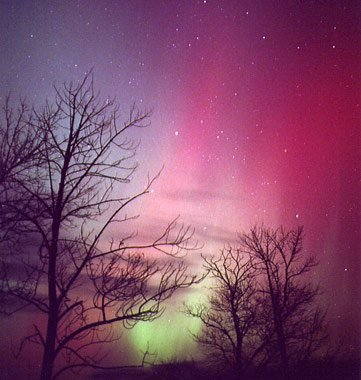
\includegraphics[width=6cm]{figures/SW_aurora_29oct_3.jpg}

\caption{Geomagnetic storm/ Aurora on the 29th of October \cite{spaceweather}.}
\label{fig:Aurora3}
\end{wrapfigure} 
In the rest of this document preprocessed data is used from the Halloween 2003 space weather event. This event took place from the 28th up to the 29th of October, with the main two peaks at 11:10 (28-10-2003) and 20:50 (29-10-2003) \cite{goes_x-ray_archive}. This solar weather event consisted of a series of solar flares and coronal mass ejections. The solar flare with the most energy was measured at 10:16:53 UCT. With an energy of $6.9\cdot10^{25}$\,Joule and a mass of $1.6 \cdot 10^{10}$\,gram \cite{CME_list}, one of the strongest ever measured by GOES.\\

Satellite-based systems and communications were affected, as well as the instruments onboard \cite{swpc-noaa}. Aircraft were advised to avoid high altitudes near the polar regions, and a one-hour-long power outage occurred in Sweden as a result of the solar activity. Auroras (figure \ref{fig:Aurora3}) were observed at latitudes as far south as Texas and the Mediterranean countries of Europe \cite{wiki_halloween_solar_stroms}.

\subsection{Solar flares}
\begin{wrapfigure}[15]{r}{0.5\textwidth}
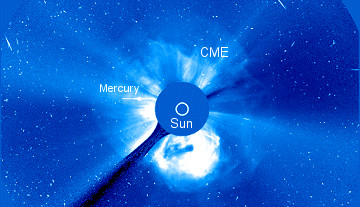
\includegraphics[width=.5\textwidth]{figures/SW_CME.jpg}

\caption{Solar image of a CME using a cronagraph\cite{spaceweather}.}
\label{fig:SW:CME}
\end{wrapfigure} 

On the 28th 12:18 UCT one of the most powerful Coronal Mass Ejections (CME) in years erupted, this eruption, that caused a intense geomagnetic storm, is shown in figure \ref{fig:SW:CME}.The solar flares erupted out of 486 giant sunspots. It was measured X17  on the Richter scale of solar flares. This means that the peak had an energy above $7 \cdot 10^{-4}$\,W/m$^2$. It was also classified as a S3 storm, which means it has a flux of more than $10^3$ with $\geq$10\,MeV particles.  \cite{spaceweather}.\\


%----------------------------------------------------------------------------------------
%	GOES.
%----------------------------------------------------------------------------------------
\subsection{GOES}
In figure \ref{fig:goes_sem_data_oct} the space weather data from GOES10 (10th Geostationary Operational Environmental Satellite) over the month October is shown. In figure \ref{fig:goes_sem_data_nov} the data from the same satellite is shown over the month of November \cite{ngdc-noaa}. \\

In the top plot the peak flux of the solar flares/ CMEs in watts per square meter (W/m$^2$) between 1 and 8 Ångströms. Based on the flux the solar flare is classified. These are the classifications:
\begin{enumerate}
	\item Class A: flux $< 10^{-7}$
	\item Class B: $10^{-7} \leq$ flux $< 0^{-6}$
	\item Class C: $10^{-6} \leq$ flux $< 0^{-5}$
	\item Class M: $10^{-5} \leq$ flux $< 0^{-4}$
	\item Class X: flux $\geq 10^{-4}$
\end{enumerate}

In the second top plot the electrons flux, directed to Earth, is shown in e$^{-}$cm$^{-}2$s$^{-1}$sr$^{-1}$. With the black line presenting electrons with an energy greater than 0.6\,MeV, red above 2\,MeV and green above 4\,MeV. In the third plot the proton flux is shown, with the energies greater than 1\,MeV for black, 5\,MeV for red, 10\,MeV for green, 30\,MeV for pink, 50\,MeV for blue, 60\,MeV purple and 100\,MeV for light blue. In the last plot the magnetic field strength in nT, where black (Hp) is the magnetic field vector component, points northward, perpendicular to the orbit plane which for a zero degree inclination orbit is parallel to Earth's spin axis. Red (He) is the magnetic field vector component, perpendicular to Hp and Hn and points earthward. Green (Hn) is the magnetic field vector component, perpendicular to Hp and He and points eastward. \\


\begin{figure}[H]
\centering
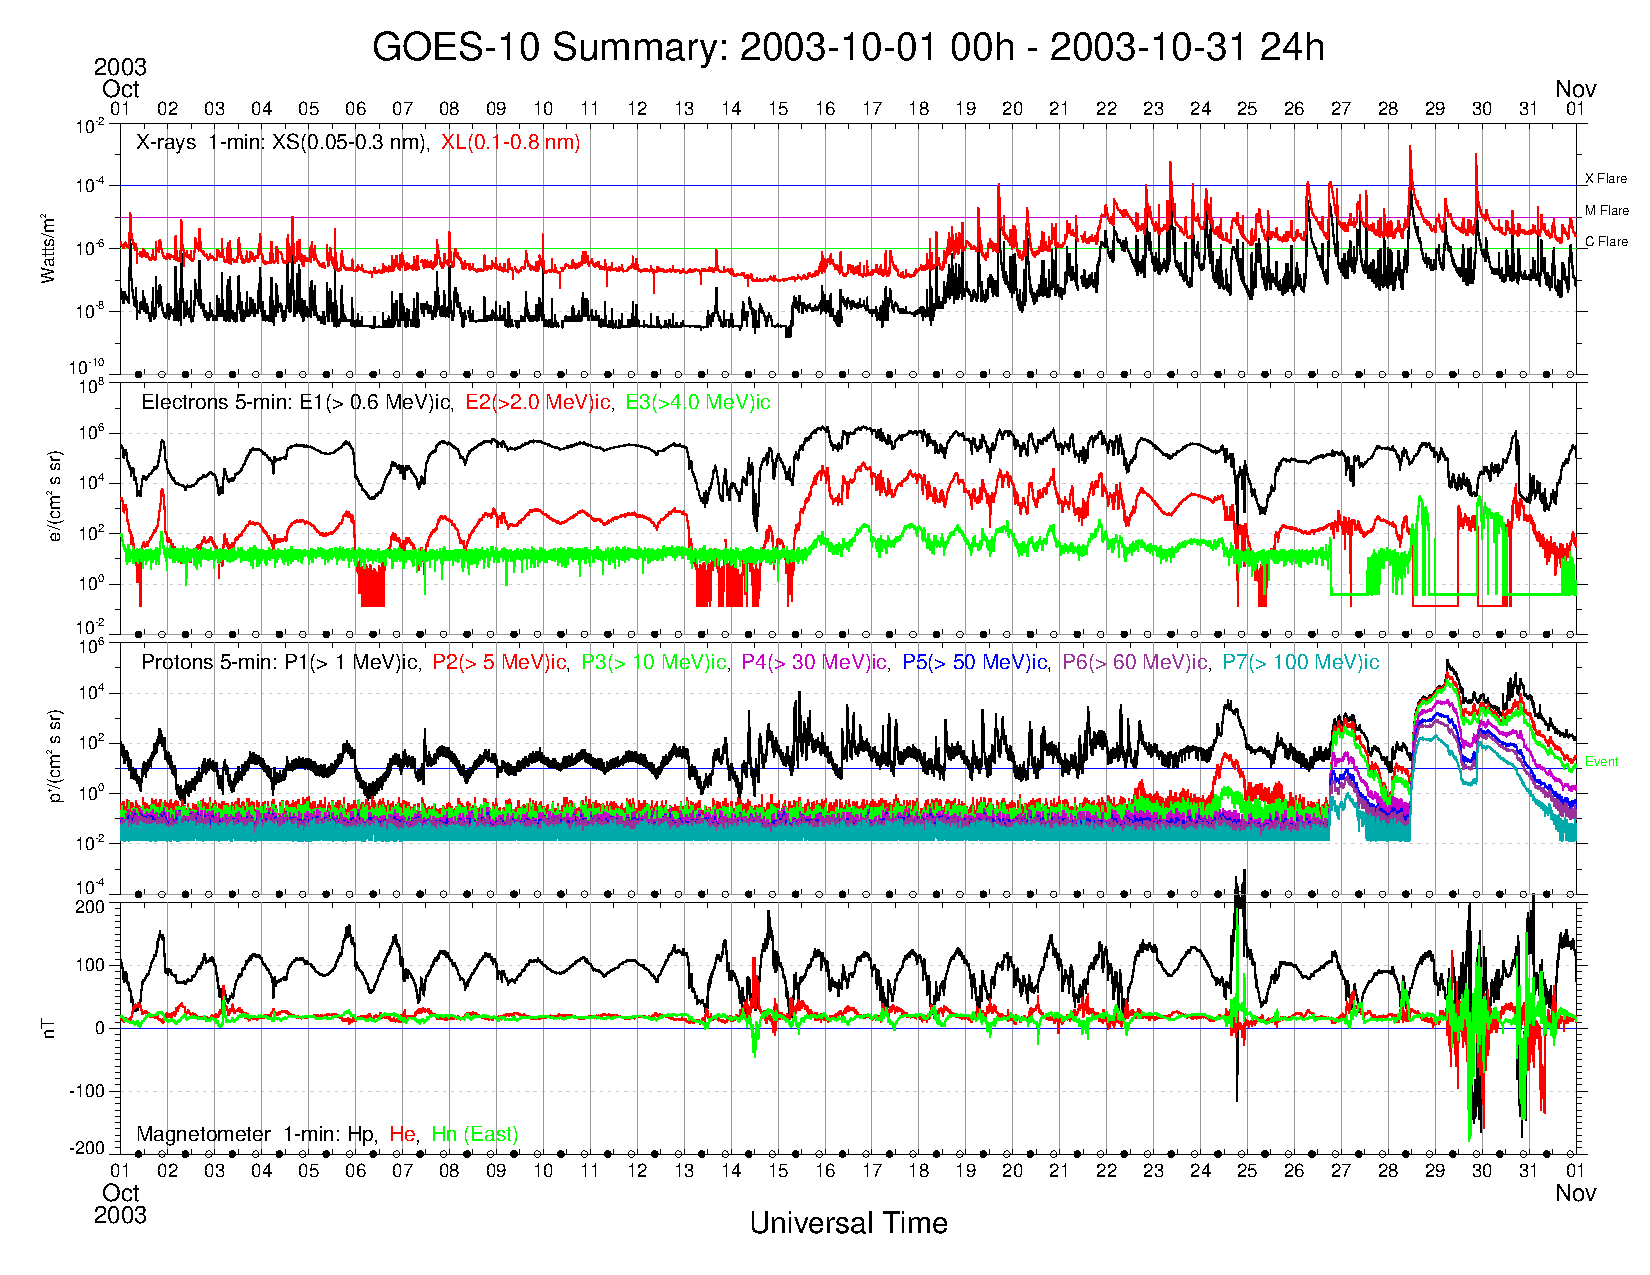
\includegraphics[page=1, width=.79\textwidth]{figures/goes10_oct.pdf}

\caption{GOES10 data from the month October 2003 \cite{ngdc-noaa}.}
\label{fig:goes_sem_data_oct}
\end{figure}

\begin{figure}[H]
\centering
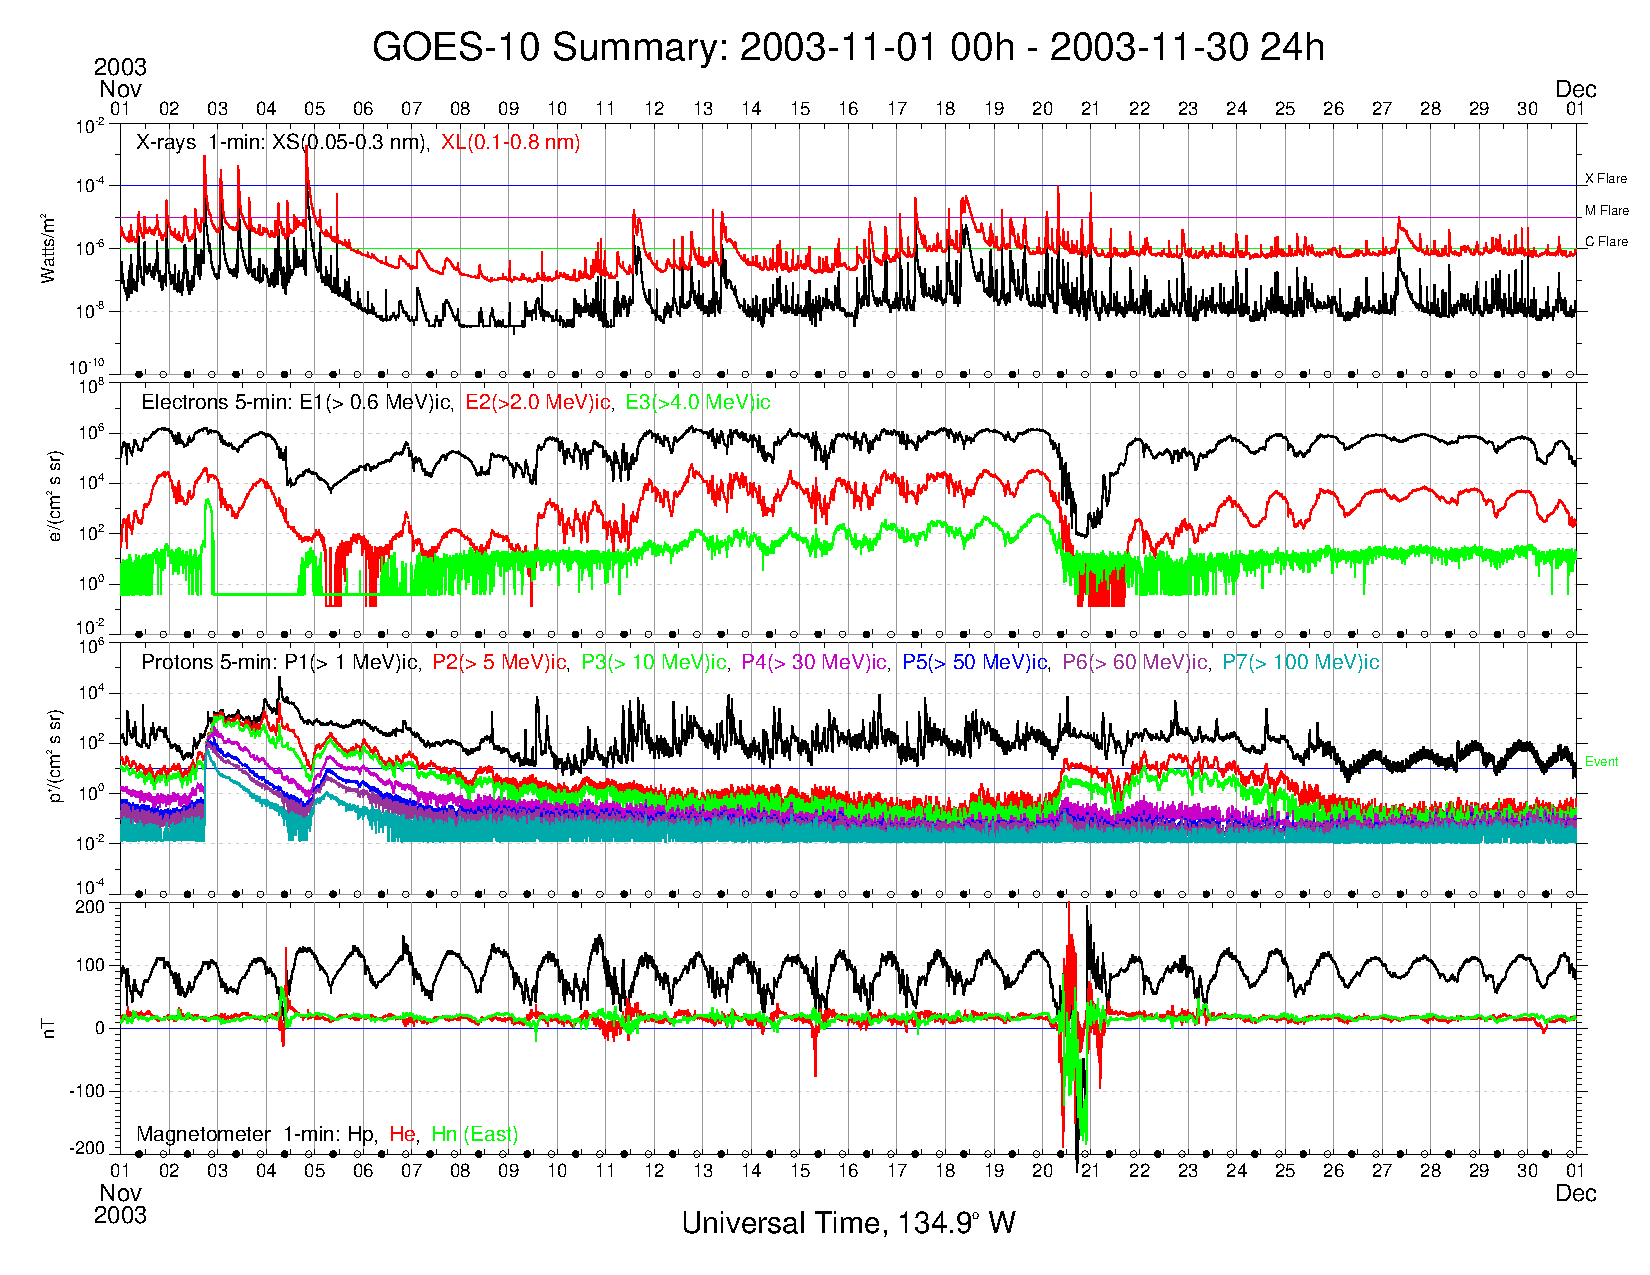
\includegraphics[page=1, width=.79\textwidth]{figures/goes10_nov.pdf}

\caption{GOES10 data from the month November 2003 \cite{ngdc-noaa}.}
\label{fig:goes_sem_data_nov}
\end{figure}

From the GOES data in figure \ref{fig:goes_sem_data_oct} and \ref{fig:goes_sem_data_nov} it can clearly be seen that the were a lot of instabilities during the end of October and the beginning of November. Starting around the 14th of October the magnetic field became more instable and the proton flux increased. On the 18th the electron flux increased, as well as the flux of energy. The main two peaks where at the 28th and 29th of October, followed by some less, but still pretty strong, flares on the 2nd, 3rd and 4th of November. After the sixth of November the fluxes went down again.


%----------------------------------------------------------------------------------------
%	IMAGE.
%----------------------------------------------------------------------------------------
\subsection{IMAGE}

In figure \ref{fig:image_grams} the magnetometer data from multiple latitudes on Earth from the 29th of October to the 1st of November is shown. These values differ from the magnetometer data from GOES due to that GOES is orbiting Earth and these magnetometers are located on a fixed position on the Earth. It can be seen that the latitudes around the Auroral oval have the largest spikes. 

\begin{figure}[H]
        \begin{subfigure}[b]{0.33\textwidth}
                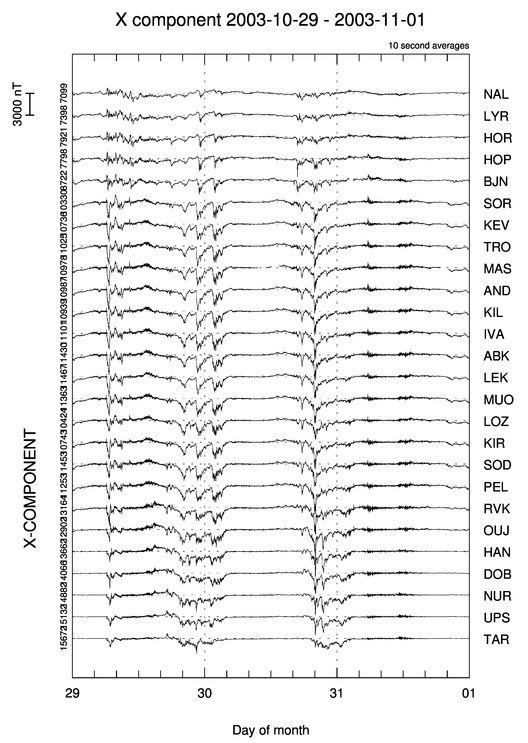
\includegraphics[width=\linewidth]{figures/IMAGE_X_gram.jpg}
                \caption{Perpendicular to the Y and Z axis (Hn) \cite{image}.}
				\label{fig:image_x_gram}
        \end{subfigure}%
        \begin{subfigure}[b]{0.33\textwidth}
                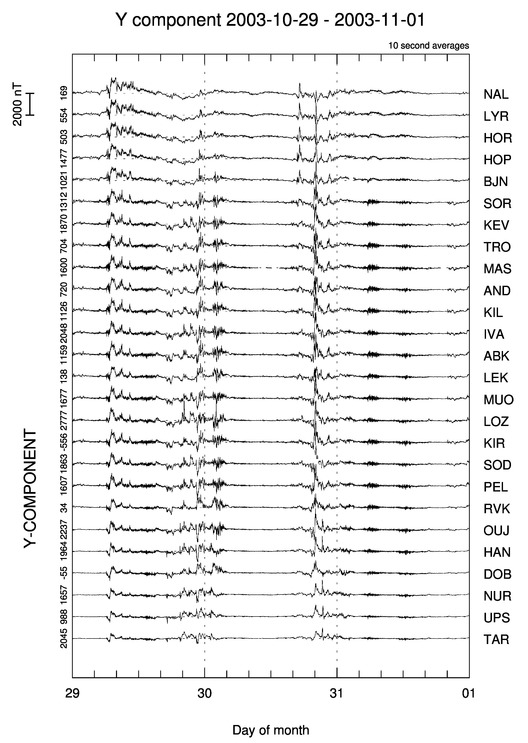
\includegraphics[width=\linewidth]{figures/IMAGE_Y_gram.jpg}
                \caption{Perpendicular to the z axis, pointing Eastward (He) \cite{image}.}
				\label{fig:image_y_gram}
        \end{subfigure}%
        \begin{subfigure}[b]{0.33\textwidth}
                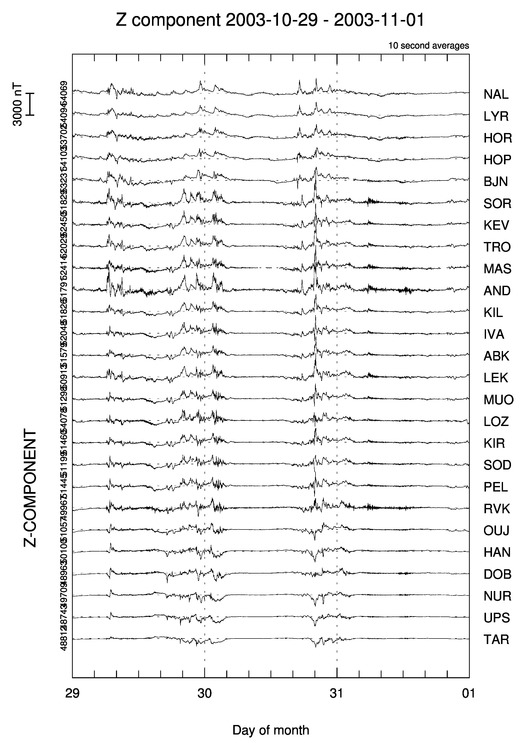
\includegraphics[width=\linewidth]{figures/IMAGE_Z_gram.jpg}
                \caption{Axis from the center of the Earth northwards (Hp)\cite{image}.}
				\label{fig:image_z_gram}
        \end{subfigure}
        \caption{Magnetogram data from IMAGE (International Monitor for Auroral Geomagnetic Effects).}
        \label{fig:image_grams}
\end{figure}



